%%
%% Consulter la documentation de la classe ulthese pour une
%% description détaillée de la classe, de ce gabarit et des options
%% disponibles.
%%
%% [Ne pas hésiter à supprimer les commentaires après les avoir lus.]
%%
%% Déclaration de la classe avec le type de grade
%%   [l'un de MATDR, MArch, MA, LLM, MErg, MMus, MPht, MSc, MScGeogr,
%%    MServSoc, MPsEd]
%% et les langues les plus courantes. Le français sera la langue par
%% défaut du document. L'option 'bibsection' permet de créer des
%% bibliographies par chapitre présentées sous forme de section
%% numérotée.
\documentclass[MSc,bibsection,english,french]{ulthese}
  %% Encodage utilisé pour les caractères accentués dans les fichiers
  %% source du document. Les gabarits sont encodés en UTF-8. Inutile
  %% avec XeLaTeX, qui gère Unicode nativement.
  \ifxetex\else \usepackage[utf8]{inputenc} \fi

  %% Charger ici les autres paquetages nécessaires pour le document.
  %% Quelques exemples; décommenter au besoin.
  %\usepackage{amsmath}       % recommandé pour les mathématiques
  %\usepackage{icomma}        % gestion de la virgule dans les nombres

  %% Utilisation d'une autre police de caractères pour le document.
  %% - Sous LaTeX
  %\usepackage{mathpazo}      % texte et mathématiques en Palatino
  %\usepackage{mathptmx}      % texte et mathématiques en Times
  %% - Sous XeLaTeX
  %\setmainfont{TeX Gyre Pagella}      % texte en Pagella (Palatino)
  %\setmathfont{TeX Gyre Pagella Math} % mathématiques en Pagella (Palatino)
  %\setmainfont{TeX Gyre Termes}       % texte en Termes (Times)
  %\setmathfont{TeX Gyre Termes Math}  % mathématiques en Termes (Times)

  %% Options de mise en forme du mode français de babel. Consulter la
  %% documentation du paquetage babel pour les options disponibles.
  %% Désactiver (effacer ou mettre en commentaire) si l'option
  %% 'nobabel' est spécifiée au chargement de la classe.
  \frenchbsetup{%
    StandardItemizeEnv=true,       % format standard des listes
    ThinSpaceInFrenchNumbers=true, % espace fine dans les nombres
    og=«, fg=»                     % caractères « et » sont les guillemets
  }

  %% Suppression du numéro de section de la bibliographie. Utilisation
  %% de \extrasfrench parce que c'est la dernière langue déclarée dans
  %% \documentclass, ci-dessus.
  %\addto\extrasfrench{%
  %  \renewcommand{\bibsection}{\section*{\bibname}\prebibhook}}

  %% Composition de la page frontispice. Remplacer les éléments entre < >.
  %% Supprimer les caractères < >. Couper un long titre ou un long
  %% sous-titre manuellement avec \\.
  \titre{<Titre principal>}
  % \titre{Ceci est un exemple de long titre \\
  %   avec saut de ligne manuel}
  % \soustitre{Sous-titre le cas échéant}
  % \soustitre{Ceci est un exemple de long sous-titre \\
  %   avec saut de ligne manuel}
  \auteur{<Prénom Nom>}
  \direction{<Prénom Nom>, <directeur ou directrice> de recherche}
  % \codirection{<Prénom Nom>, <codirecteur ou codirectrice> de recherche}
  % \codirection{<Prénom Nom>, <codirecteur ou codirectrice> de recherche \\
  %              <Prénom Nom>, <codirecteur ou codirectrice> de recherche}

  %% Les commandes ci-dessous servent uniquement pour la création
  %% d'une page de titre (interdite lors du dépôt à la FESP).
  % \annee{<20xx>}

\begin{document}

\frontmatter                    % pages liminaires

\frontispice                    % production de la page frontispice

% !TEX encoding = UTF-8 Unicode
\chapter*{Résumé}               % ne pas numéroter
\label{chap-resume}             % étiquette pour renvois
\phantomsection\addcontentsline{toc}{chapter}{\nameref{chap-resume}} % inclure dans TdM

\begin{otherlanguage*}{french}
% With help from Alex
Les changements dans les propriétés du minerai apportent des défis pour le contrôle des broyeurs semi-autogènes (\acrshort{SAG}) car ils sont généralement difficiles à mesurer en temps réel et ont des impacts significatifs sur le procédé. Bien qu'il y ait un manque de compréhension de la nature des variations des propriétés du minerai dans les opérations réelles, les données disponibles sur la distribution granulométrique indiquent qu'elles sont caractérisées par des changements abrupts et des comportements en rampe, pour lesquels les modèles de perturbation standard utilisés dans le contrôle des procédés ne sont pas conçus.

Dans ce travail, un modèle de perturbation déterministe se produisant de manière aléatoire (\textit{randomly-occurring deterministic disturbances} ({\acrshort{RODD}}s)) est considéré. Celui-ci possède une entrée commutant entre deux bruits aléatoires. Puisque la perturbation n’est pas gaussienne, un filtre de Kalman standard, qui est généralement utilisé pour l’estimation d’état, n’est pas optimal. Les capacités de deux observateurs à modèles multiples de détecter et d’estimer les états de systèmes soumis à des RODD non mesurés sont évaluées. Ces observateurs maintiennent plusieurs estimations des états du système sur la base de différentes hypothèses sur la commutation de la perturbation. La vraisemblance de chaque hypothèse compte tenu des mesures disponibles est évaluée et utilisée pour produire une meilleure estimation des états et de la sortie du procédé, qui demeure toutefois sous-optimale.

Deux types d’observateurs à modèles multiples sous-optimaux sont évalués et comparés à un filtre de Kalman standard en utilisant des mesures de bruit simulées à partir de trois systèmes différents—un système linéaire avec un RODD et une sortie, un système linéaire avec deux RODD et deux sorties, et une simulation réaliste d’un circuit de broyage avec une mesure de sortie et une alimentation commutant entre deux types de minerai.

Les résultats montrent que les observateurs à modèles multiples détectent et réagissent rapidement aux changements instantanés de la perturbation, sans pour autant avoir une sensibilité accrue au bruit lorsqu’en régime permanent.  Cela suggère que des modèles plus réalistes de perturbations du minerai alimenté et une meilleure estimation en temps réel des changements dans les propriétés du minerai pourraient améliorer le contrôle du procédé, bien que les gains par rapport à un filtre unique de Kalman dépendent du niveau du bruit de mesure.

% Removed as suggested by Eric
%Des modèles plus réalistes des perturbations des propriétés du minerai alimenté pourraient avoir des avantages significatifs en termes de contrôle amélioré et de variabilité réduite des variables de procédés. Cependant, des travaux supplémentaires sont nécessaires pour caractériser les perturbations réelles, pour déterminer si les modèles de perturbation peuvent être identifiés en pratique et pour estimer les avantages potentiels dans les performances de contrôle des procédés.
\end{otherlanguage*}
                % résumé français
% !TEX encoding = UTF-8 Unicode
\chapter*{Abstract}             % ne pas numéroter
\label{chap-abstract}           % étiquette pour renvois
\phantomsection\addcontentsline{toc}{chapter}{\nameref{chap-abstract}} % inclure dans TdM

\begin{otherlanguage*}{english}
  
Changes in ore properties create challenges for the control of semi-autogenous grinding (\acrshort{SAG}) mills because they are generally difficult to measure in real time and have significant impacts on the grinding process. Although there is a lack of understanding of the nature of variations in ore properties in real operations, available data on the particle size distribution indicates that they are characterised by abrupt step changes and ramp behaviours, which standard disturbance models used in process control are not designed for.

In this work, an alternative disturbance model known as the randomly-occurring deterministic disturbance ({\acrshort{RODD}}) is considered. This has a switching random noise input, which makes it suitable for modelling these types of disturbances. However, since the noise is non-Gaussian, a standard Kalman filter, which is typically used for state estimation, is not optimal. The capabilities of two multiple-model observers to detect and estimate the states of systems subjected to unmeasured {\acrshort{RODD}}s are evaluated. These observers maintain multiple estimates of the system states based on different hypotheses about the switching of the disturbance. The likelihood of each hypothesis given the available measurements is estimated and used to produce a better, although still sub-optimal, estimate the process states and output.

Two types of sub-optimal multiple-model observer are evaluated and compared to a standard Kalman filter using simulated noisy measurements from three different process systems---a linear system with one {\acrshort{RODD}} and one output, a linear system with two {\acrshort{RODD}}s and two-outputs, and a realistic grinding process simulation with a switching ore feed and one output measurement.

The results show that the multiple-model observers detect and respond quickly to step changes in the disturbance, without having a compromised sensitivity to noise during steady-state. This suggests that more realistic models of ore feed disturbances and improved real-time estimation of changes in ore properties could have benefits in terms of improved process control, although the improvement compared to a single Kalman filter was found to depend on the magnitude of the measurement noise.
% Removed as suggested by Eric
%  More realistic models of ore feed disturbances and improved real-time estimation of changes in ore properties could have significant benefits in terms of improved control and reduced variation in process variables. However, more work is needed to characterize real disturbances, to determine if the disturbance models can be identified in practice, and to estimate the potential benefits in process control performance.
\end{otherlanguage*}
              % résumé anglais
\cleardoublepage

\tableofcontents                % production de la TdM
\cleardoublepage

\listoftables                   % production de la liste des tableaux
\cleardoublepage

\listoffigures                  % production de la liste des figures
\cleardoublepage

\dedicace{<Dédicace si désiré>}
\cleardoublepage

\epigraphe{<Texte de l'épigraphe>}{<Source ou auteur>}
\cleardoublepage

% !TEX encoding = UTF-8 Unicode
\chapter*{Remerciements}        % ne pas numéroter
\label{chap-remerciements}      % étiquette pour renvois
\phantomsection\addcontentsline{toc}{chapter}{\nameref{chap-remerciements}} % inclure dans TdM

<Texte des remerciements en prose.>

% DRAFT
%I thank my supervisors, André and Jocelyn, for their unwavering availability, patience, and dedication to my learning and to the success of the research. I am also indebted to my colleagues at Laval University for their continuous support, good humour, and encouragement over the last two years.         % remerciements
\chapter*{Avant-propos}         % ne pas numéroter
\label{chap-avantpropos}        % étiquette pour renvois
\phantomsection\addcontentsline{toc}{chapter}{\nameref{chap-avantpropos}} % inclure dans TdM

<Texte de l'avant-propos. Obligatoire dans une thèse ou un mémoire par
articles.>
           % avant-propos

\mainmatter                     % corps du document

\chapter*{Introduction}         % ne pas numéroter
\label{chap-introduction}       % étiquette pour renvois
\phantomsection\addcontentsline{toc}{chapter}{\nameref{chap-introduction}} % inclure dans TdM

% Note: This is an un-numbered chapter.

\begin{itemize}
	\item Challenges of effective control and optimization of comminution (grinding) operations.
	\item Disturbances, e.g. Changes in ore properties — difficult to measure accurately in real time, impacts on the downstream process and control systems can be severe (Herbst et al., 1988).
	\item Cause-effect: Variable ore → variable operation → variable grind → variable recovery → lower recovery (Powell et al., 2009).
	\item Sources of variability in mining operations: geological characteristics of ore bodies, mining processes such as blasting, material handling, shovelling and trucking. Segregation effects.

\item Motivation: better characterization of disturbances in real operations, better models, more realistic simulation models, better observer designs to detect and estimate disturbances in real time.
\item Many potential benefits: Improve process control performance. disturbance rejection. adaptive control. Robustness (maintain operating conditions within stable region—SAG mill) and improve process performance.
\item Use in upstream in the mining operation to help determine the source of variation and identify process improvements.
\end{itemize}

\section*{Disturbances}

\begin{itemize}
	\item Definition of a disturbance —uncontrolled inputs, usually unmeasured.
	\item Measured v. unmeasured— anticipation, feed-forward control
	\item Importance of considering disturbances in control system design
	\item Disturbance models and process observers
	\item Disturbances in mineral processing
	\item Ore feed properties—particle size distribution, hardness, density
	\item Effects on grinding and downstream separation processes (e.g. flotation)
	\item Two categories of disturbances: In-frequent, always-present disturbances.
	\item Infrequent disturbances could have significant impact on process and control systems.
	\item Standard approaches to system identification do not consider infrequent disturbances
	\item (focus on second order properties)
\end{itemize}


\section*{Literature review}

\begin{itemize}
	\item Herbst et al (1984) - optimal control potential in grinding
	\item Wei and Craig (2009) - control survey
	\item Powell, Mainza (2009)
	\item Hoduoin et al. - DYNAFRAG simulator, did a survey of control also?
	\item Effects of ore properties on grinding performance
	\item SAG mill constraints - grate, throughput, residence time, power, etc.
	\item AG effects (e.g. Hahne, Palsson, Samskog, 2002)
	\item Attempts to design process observers — e.g. LeRoux - EKF observer (2016)
	\item MacGregor et al (1985)
	\item Reference standard approaches to disturbance model design for MPC?  E.g. Badgewell and Muske, Pannochia.
	\item Andersson (1985)
	\item Gustaffson (1993)
	\item Robertson et al (1995, 1998)
	\item Eriksson and Isaksson (1996)
	\item Wong and Lee (2006, 2009).
	\item Branch of research on fault/anomaly detection (Willsky) and limitations vs. state estimation of switching systems.
	\item Papers on state estimation... Blom and Bar Shalom, Ackerson and Fu, Busbaum and Haddad, Jaffer and Gupta, Akashi and Kumamoto,
	\item Hybrid systems (e.g. Sworder and Boyd)
	\item Discrete time Markov Jump Linear systems (MJLS) (Costa 2005 book)
	\item Bemporad on identification of switching systems (e.g. mixed-integer programming)
	\item Problems of observability and Identifiability of Jump Linear Systems (Vidal et al. 2002).
	\item Control of processes subject to intermittent disturbances. Macgregor, Costa book, Wong and Lee (2000).
	
	\item What about commercial simulation software (e.g. IDEAS)?  What disturbances do they simulate?
\end{itemize}


\section*{Research objectives}

<Text>


\section*{Contributions of this research}

<Text>


\section*{Organisation of this report}

<Text>
          % introduction
\include{chapitre1-articles}    % chapitre 1
\chapter{<Titre du chapitre ou de l'article>}     % numéroté
\label{chap-}                   % étiquette pour renvois (à compléter!)

\section{Résumé}

\begin{otherlanguage*}{french}
  <Résumé de l'article en français. Obligatoire.>
\end{otherlanguage*}

\section{Abstract}

\begin{otherlanguage*}{english}
  <English abstract of the paper. Optional, but recommended.>
\end{otherlanguage*}

<Texte du chapitre ou de l'article.>

\bibliographystyle{}              % style de la bibliographie
\bibliography{}                   % production de la bibliographie
    % chapitre 2, etc.
% !TEX encoding = UTF-8 Unicode
\chapter*{Conclusion}           % ne pas numéroter
\label{chap-conclusion}         % étiquette pour renvois
\phantomsection\addcontentsline{toc}{chapter}{\nameref{chap-conclusion}} % inclure dans TdM

\textbf{NOT COMPLETE}

\begin{itemize}
	\item Summarize results
	\item Summarize issues/drawbacks and potential ways to mitigate them.
	\item Identify gaps and suggest areas of further research/data collection.
	\item Reiterate potential benefits and need to quantify these.
\end{itemize}

% Text from IFAC paper
While the multi-model observer has a number of clear advantages over a single Kalman filter, its limitations are important to recognize. Firstly, the higher variance of the noise model during the transitions, which is needed for a fast response, also increases the variance of the estimates during these periods, resulting in larger errors---46\% higher than those of KF3 during transition periods.

Secondly, the multiple-model algorithm is limited to infrequently-occurring disturbances where the disturbance model is known. Finally, the complexity of the algorithm is a significant disadvantage from the perspective of practical implementation.




            % conclusion

\appendix                       % annexes le cas échéant

\chapter{Additional results and sensitivity analysis}     % numérotée
\label{chap-Annex}                   % étiquette pour renvois (à compléter!)

\section{Multiple model observer algorithms}

\begin{itemize}
	\item Multi-model algorithm.
\end{itemize}

\section{Tuning of sequence fusion algorithm 1995 variant}

The sequence fusion algorithm evaluated in section \ref{section:sim-obs-lin} is based on \cite{robertson_method_1998}. However, Robertson and coworkers published results in 1995 \citep{robertson_detection_1995} using a slightly different version of this algorithm. Table \ref{tb:obs-sim1-popt-SF95} shows the results of a parameter search for the earlier version of the algorithm using the same simulation data used to tune the 1998 algorithm.

\begin{table}[hb]
	\begin{center}
		\caption{Multi-model observer parameter search results – MMKF-SF95.} \label{tb:obs-sim1-popt-SF95}
		% See: https://texblog.org/2019/06/03/control-the-width-of-table-columns-tabular-in-latex/
		\begin{tabular}{p{0.05\textwidth}>{\centering\arraybackslash}p{0.07\textwidth}>{\centering\arraybackslash}p{0.07\textwidth}>{\centering\arraybackslash}p{0.07\textwidth}>{\centering\arraybackslash}p{0.07\textwidth}>{\centering\arraybackslash}p{0.24\textwidth}}
			$n_f$ & $n_m$ & $n_d$ & $n_h$ & $\beta$ & $\text{RMSE}(\hat{Y}_i(N),Y_i(N))$  \\
			\hline
			% Results with seed = 6, nT = 5000
			15 &   1 &   3 &   6 & 0.9035 & 0.1156 \\
			15 &   2 &   3 &  16 & 0.9044 & 0.1156 \\
			15 &   3 &   3 &  26 & 0.9044 & 0.1156 \\
			15 &   1 &   1 &  16 & 0.9904 & 0.1168 \\
			15 &   2 &   1 & 121 & 0.9996 & 0.1168 \\
			15 &   1 &   5 &   4 & 0.8861 & 0.1186 \\
			15 &   2 &   5 &   7 & 0.8864 & 0.1186 \\
			15 &   3 &   5 &   8 & 0.8864 & 0.1186 \\
			9 &   3 &   3 &   8 & 0.9415 & 0.1188 \\
			9 &   2 &   3 &   7 & 0.9415 & 0.1188 \\
			\hline
		\end{tabular}
	\end{center}
\end{table}

From these results it can be seen that the parameter tunings are quite similar to those in Table \ref{tb:obs-sim1-popt-SF} for the 1998 variant of the algorithm. However, the best RMSE value achieved by the 1995 algorithm (0.1156) is slightly higher than the best achieved by the 1998 variant (0.1089) in this case.

Figure \ref{fig:rod-obs-sim1-yest-all-seed-RMSE-box-SF95} shows the results of both observers on different pseudo-random simulation results. This supports the finding by Robertson et al. that the 1998 variant of the algorithm performs better.

\begin{figure}[htp]
	\centering
	\includegraphics[width=12cm]{images/rod_obs_sim1_all_seed_y_err_box_SF95.pdf}
	\caption{Comparison of sequence fusion algorithm variants}
	\label{fig:rod-obs-sim1-yest-all-seed-RMSE-box-SF95}
\end{figure}



\section{Tuning of KF3 for MIMO linear system} \label{section:annex-sim-2-KF-tuning}

As described in Chapter \ref{chap-simulation}, a standard Kalman filter was tuned to minimize the RMSE of the output estimates using 5000 data samples from the $2\times2$ linear system. Since the system is symmetrical and the two RODDs have the same parameters, it was assumed that the two observer parameters, $\sigma_{w_p,1,\text{opt}}$ and $\sigma_{w_p,2,\text{opt}}$ must also be identical. This assumption simplified the search process since only one optimum value needed to be found.

Figure \ref{fig:sim-sys-2x2-KF3-tuning-sens} shows the variation in the RMSEs of the four model state estimates with the parameters. In this case, the choice of optimal parameter value was not as straight-forward as in the case of the SISO system with one RODD. The minimum RMSE for each state occurs at different values of  1 and 2 is achieved when $\sigma_{w_p,1,\text{opt}}=\sigma_{w_p,2,\text{opt}}=0.0075$

\begin{figure}[htp]
	\centering
	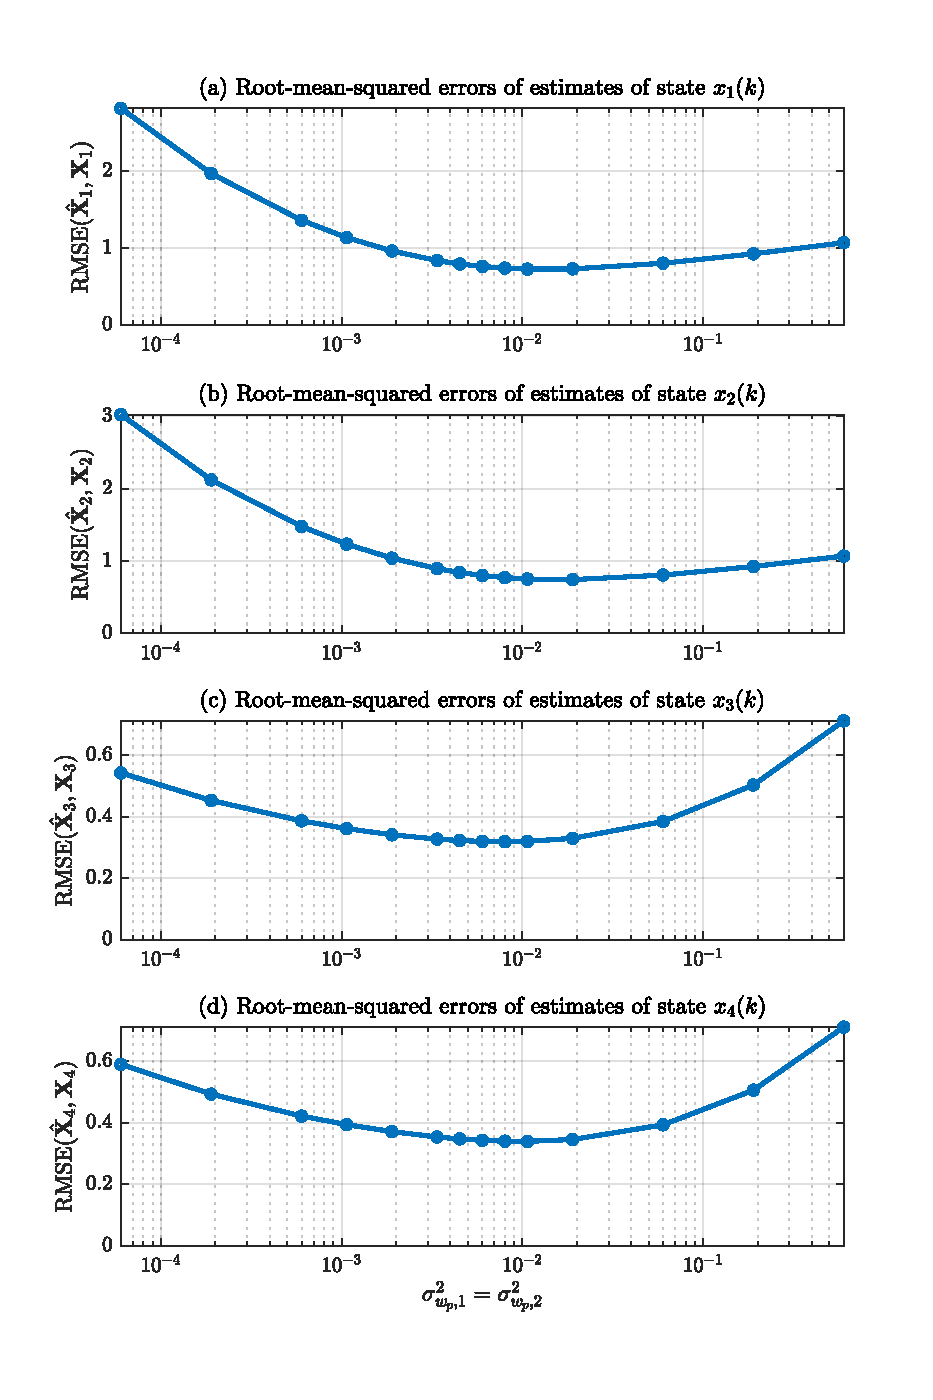
\includegraphics[width=14cm]{images/rod_obs_sim2_3KF_Q_seed_0.pdf}
	\caption{Tuning of Kalman filter KF3 – $2\times2$ system}
	\label{fig:sim-sys-2x2-KF3-tuning}
\end{figure}
	

\section{Sensitivity analyses}

\subsection{Pseudo-random numbers}

Many of the simulation results are sensitive to the initialization of the pseudo-random number generator (PRNG) used to simulate random processes. In particular, the RODD step disturbance (\ref{eq:wpk2}) is simulated by generating three pseudo-random sequences, two random noise sequences and a random binary sequence to simulate the infrequent shocks.  Since the random shocks are infrequent and tend to have a large magnitude, their effect on the simulation results can be significant.

To visualize this effect, consider the plot in Figure \ref{fig:rod-obs-sim-1-3KF-seed-crmse-statsplot}. This shows the RMSE of the output estimates of the three Kalman filters described in Section \ref{sim-obs-lin-1} for 10 simulations, each generated with a different \textit{seed}—the seed is a scalar argument used to initialize the PRNG algorithm in a unique state. The RMSE is calculated for every simulation duration, $t_N=0.5,1,1.5,...,2500$. The coloured areas represent the range between the lowest and the highest RMSE obtained for the 10 different simulations of each duration. The dark lines represent the median values.

\begin{figure}[htp]
	\centering
	\includegraphics[width=14cm]{images/rod_obs_sim1_3KF_seed_crmse_statsplot.pdf}
	\caption{Effect of random variables on the RMSE results.}
	\label{fig:rod-obs-sim-1-3KF-seed-crmse-statsplot}
\end{figure}

As expected, the differences in the results due to PRNG initialization are smaller the greater the length of the simulation. However, the magnitude of the differences is not the same for each observer. The RMSE values of KF1, which has the lowest gain, are more sensitive to the random initialization than the other two filters. Therefore it is not possible to estimate the expected value of the RMSE of KF1 from a single simulation of this duration---a longer simulation or a larger number of simulations would be needed. On the other hand, the variations in the RMSEs of KF2 and KF3 are significantly lower. After the full length of the simulations ($t_N=2500$), the RMSE of KF2 is between -0.0039 (-2.5\%) and 0.0019 (1.3\%) of the median value, which is $0.1550$.  That of KF3 is between -0.0035 (-4.0\%) / 0.0047 (5.3\%) of the median, 0.0889.  Therefore it is reasonable to conclude that the RMSE of KF3 is consistently about 0.05 lower than that of KF2. Note that the RMSEs of KF2 and KF3 reported in Section \ref{sim-obs-lin-1} are \alert{0.XXXX} and \alert{0.XXXX}. These values are both within the minimum and maximum values from this sensitivity analysis (in fact, the simulation output used to produce the main results is one of the 10 shown here).

A similar sensitivity analysis was carried out on the results of the Kalman Filter tuning shown in Figure \ref{eq:sim-sys-siso-KF3-Q}, where KF3 was tuned using a set of 5000 input-output samples from the system. Figure \ref{fig:sim-sys-siso-KF3-sensitivity} shows the variation in this result when ten different sets of pseudo-random simulation data are used.  Although there is considerable variation in the RMSE values for each parameter value, the best overall choice of $\sigma_{w_p}$ to achieve the lowest average error across all 10 simulations was found to be the same as that of the single simulation (0.01).

\begin{figure}[htp]
	\centering
	\includegraphics[width=14cm]{images/rod_obs_sim1_3KF_Q_statplot.pdf}
	\caption{Sensitivity of Kalman filter tuning – SISO system}
	\label{fig:sim-sys-siso-KF3-sensitivity}
\end{figure}

Figure \ref{fig:sim-sys-2x2-KF3-tuning-sens} shows the results of a similar sensitivity analysis on the results presented in Figure \ref{fig:sim-sys-2x2-KF3-tuning}.

\begin{figure}[htp]
	\centering
	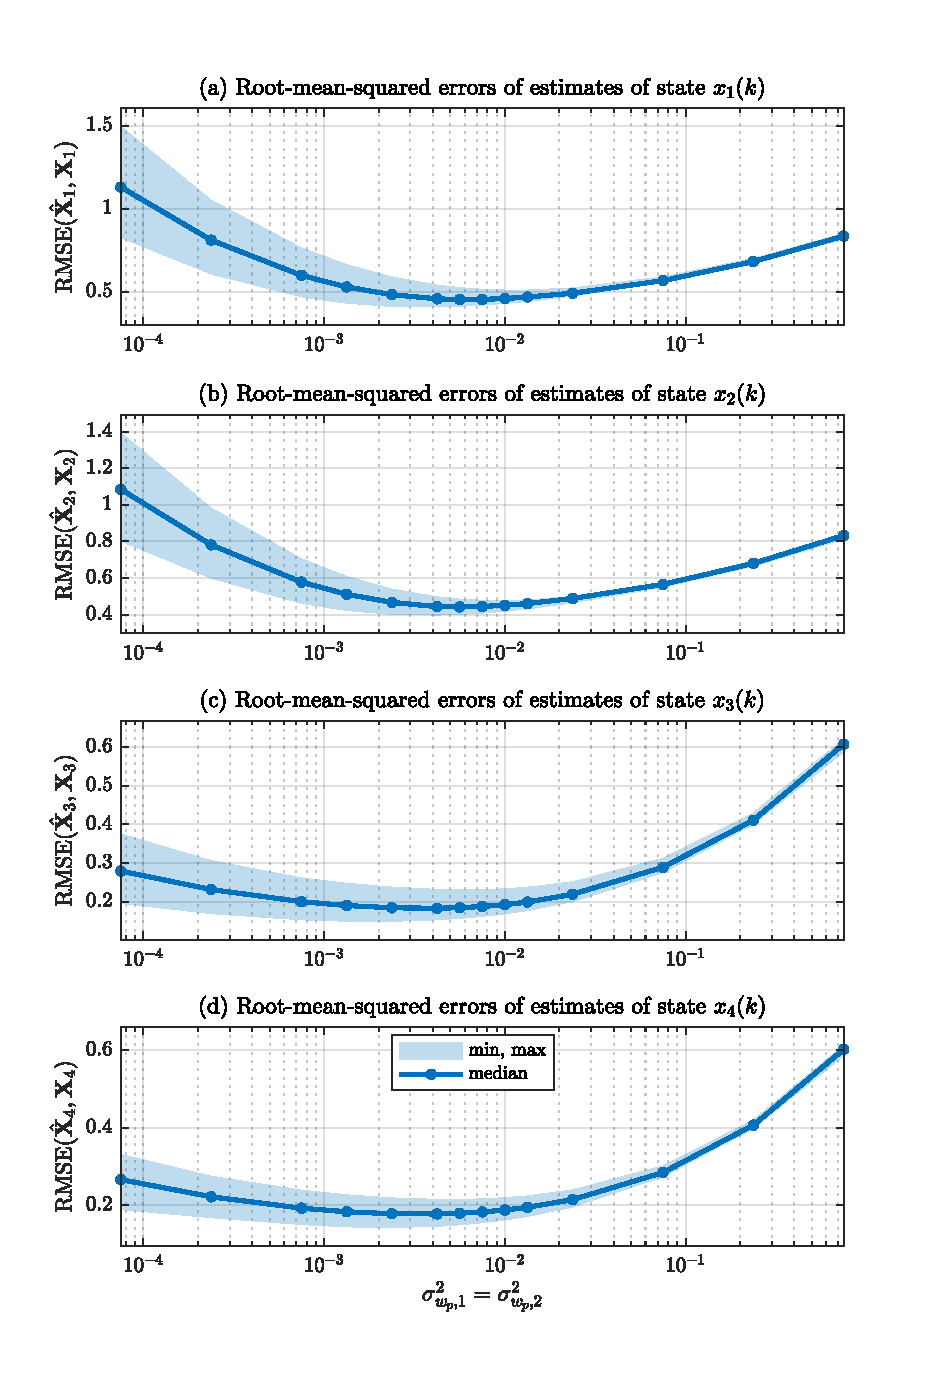
\includegraphics[width=14cm]{images/rod_obs_sim2_3KF_Q_statplot.pdf}
	\caption{Sensitivity of Kalman filter tuning – $2\times2$ system}
	\label{fig:sim-sys-2x2-KF3-tuning-sens}
\end{figure}

                % annexe A

\end{document}
